\documentclass[11pt,oneside,a4paper]{article}
\usepackage{graphicx}
\usepackage{booktabs}
\usepackage{caption}
\usepackage{subcaption}
\usepackage{amsmath}
\usepackage{amsfonts}
\usepackage{amssymb}
\usepackage{lscape}
\usepackage{psfrag}
\usepackage[usenames]{color}
\usepackage{bbm}
\usepackage[update]{epstopdf}
\usepackage[bookmarks,pdfstartview=FitH,a4paper,pdfborder={0 0 0}]{hyperref}
\usepackage{verbatim}
\usepackage{listings}
\usepackage{textcomp}
\usepackage{fancyhdr}
\usepackage{multirow}
\usepackage{tikz}
\usepackage{lipsum}
\usepackage{xcolor}
\usepackage{wrapfig}
\usepackage[margin=1in]{geometry}
\newcommand{\hint}[1]{{\color{blue} \em #1}}

\makeatletter
\def\cleardoublepage{\clearpage\if@twoside \ifodd\c@page\else%
\hbox{}%
\thispagestyle{empty}%
\clearpage%
\if@twocolumn\hbox{}\clearpage\fi\fi\fi}
\makeatother

\sloppy
% \widowpenalty=10000
% \clubpenalty=10000

\title{
    \vspace*{0.0mm}
    \LARGE\bf\sf Advanced Topics in \\Communication Networks (Fall 2019)
    \vspace*{10.0mm} \\
    %
    \Huge\bf\sf Summary
    %
    \vspace*{30.0mm} \\
    \normalsize
    %
    \sf Author:\\[5pt]
    \sf Yannick Merkli\\ [5pt]
    \sf \pageref{lastpage} Pages
}
\date{}

\begin{document}

\maketitle
\thispagestyle{empty}
\raggedbottom
\clearpage

\pagenumbering{roman}

\clearpage
\setcounter{tocdepth}{2}
\tableofcontents
\clearpage
\pagenumbering{arabic}

\section{Introduction}

Networking is on the verge of a paradigm shift towards deep programmability.

\subsection{The network managment crisis}
Networks are large distributed systems running a set of distributed algorithms. These algorithms produce the forwarding state which drives IP traffic to its destination. Operators adapt their network behavior by configuring each network device individually. This is extremely tedious and error-prone with a single mistyped line being enough to bring down an entire network (fat-thumbing). Further, the complexity in networks keeps increasing with more and more protocols appearing, a lot of which are badly documented (read an RFC and find out).

\subsection{Software-defined networking (SDN)}

SDN tries to design network control and is predicated around two simple concepts: (1) Separate the control-plane from the data-plane. (2) Provide an API to directly access the data-plane.\\
In traditional computer networks, each networked device has a local control-plane. SDN allows to have a central control-plane, controlling multiple networked devices at once. This has several advantages: (1) Simpler management, (2) Faster pace of innovation, (3) Easier interoperability, (4) Simpler, cheaper equipment. Having a common open, vendor-agnostic interface enables a control plane to control forwarding devices from different hardware and software vendors. OpenFlow does exactly this: OpenFlow is essentially an API to a switch flow table. The OpenFlow interface started simple, with the abstraction of a single table of rules that could match packets on a dozen header fields (e.g., MAC addresses, IP addresses, protocol, TCP/UDP port numbers, etc.). Over the past five years, the specification has grown increasingly more complicated, with many more header fields and multiple stages of rule tables, to allow switches to expose more of their capabilities to the controller. So essentially, the OpenFlow protocol became too complex.

\subsection{Deep network programmability}

Deep network programmability tries to adopt the good ideas of OpenFlow while solving its shortcomings. OpenFlow's problem is that it's  not flexible enough for a highly dynamic environment such as networking, with constantly changing protocols and specifications.
Future switches should support flexible mechanisms for parsing packets and matching header fields, allowing controller applications to leverage these capabilities through a common, open interface. Recent chip desings show that such flexibility can be achieved in custom ASICs at terabit speeds.

\begin{figure}[hb]
	\centering
	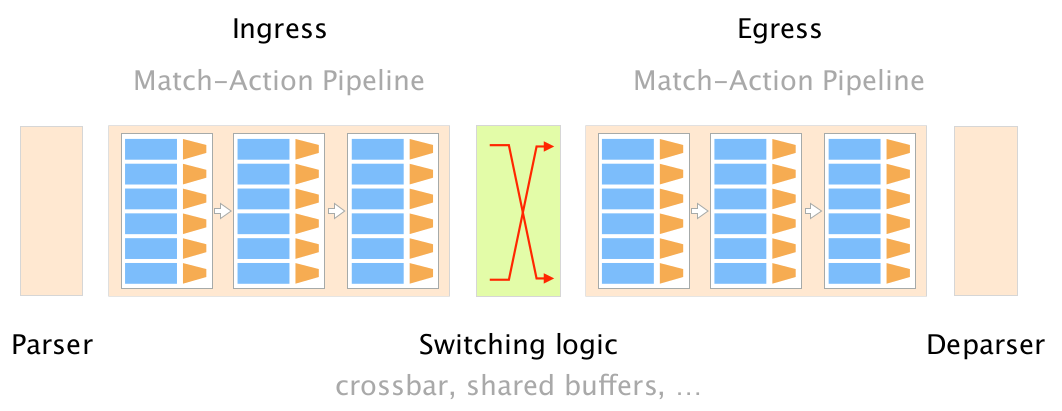
\includegraphics[width=0.75\textwidth,scale=1]{figures/PISA}
	\caption{Protocol Independent Switch Architecture (PISA) for high-speed programmable packet forwarding. \cite{advnet}}
	\label{fig:PISA}
\end{figure}

\newpage

\begin{figure}%[hb]
	\centering
	\begin{subfigure}[t]{.5\textwidth}
		\centering
		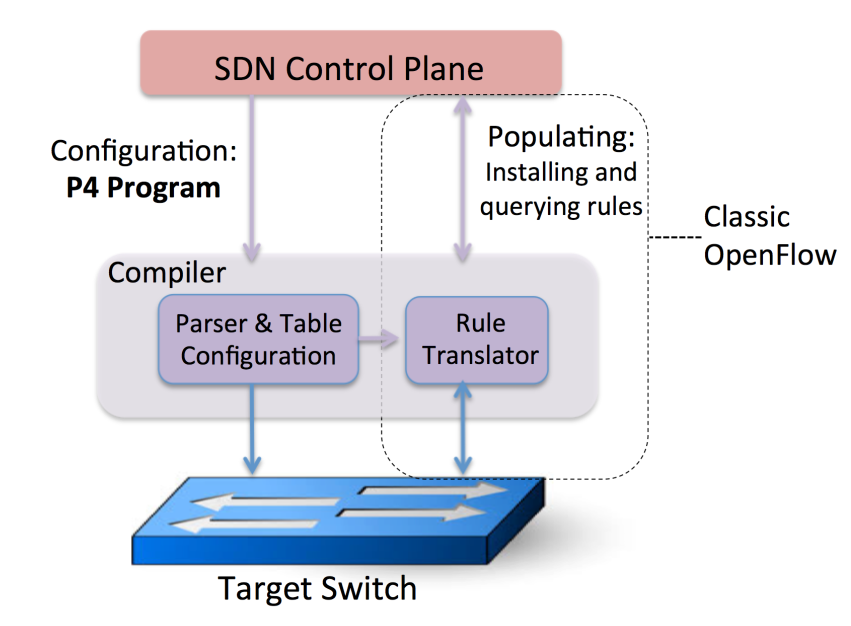
\includegraphics[width=\linewidth]{figures/P4_overview}
		\label{fig:P4_overview}
	\end{subfigure}%
	\begin{subfigure}[t]{.5\textwidth}
		\centering
		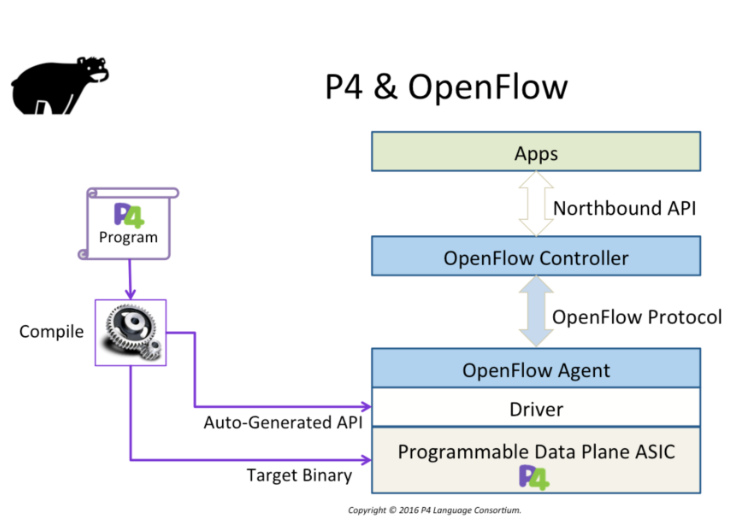
\includegraphics[width=\linewidth]{figures/P4_openflow}
		\label{fig:P4_openflow}
	\end{subfigure}
	\caption{P4 is a language to configure switches. \cite{bosshart2014p4}}
\end{figure}


Each chip has its own low-level interface, however this might vary for different hardware. Ideally we would want a higher-level language which can be used to configure a switch. This is exactly what P4 (Programming Protocol-independent Packet Processors) does: P4 is a higher-level language which is used to configure a switch, telling it how packets are to be processed. P4 can further be used with existing APIs (such as OpenFlow) that are designed to populate the forwarding tables in fixed function switches.

\section{The P4 programing language}

P4 raises the level of abstraction for programming the network, and can serve as a general interface between the controller and the switches. As such, P4 tries to achieve the following three main goals:
\vspace{-\topsep}
\begin{itemize}
	\setlength{\itemsep}{0pt}
	\setlength{\parskip}{0pt}
	\item Reconfigurability. The controller should be able to redefine the packet parsing and processing in the field.
	\item Protocol independence. The switch should be able to specify (i) a packet parser (ii) a collection of match-action tables that process theses headers.
	\item Target independence. The P4 program should run on various hardware with the compiler producing the target-dependent program.
\end{itemize}
\vspace{-\topsep}

\noindent A P4 program consists of three basic parts: Parser, match-action pipeline, deparser. In this course, we rely on a simple $P4_{16}$ switch architecture (v1model).

\begin{figure}[hb]
	\centering
	\begin{subfigure}[t]{.5\textwidth}
		\centering
		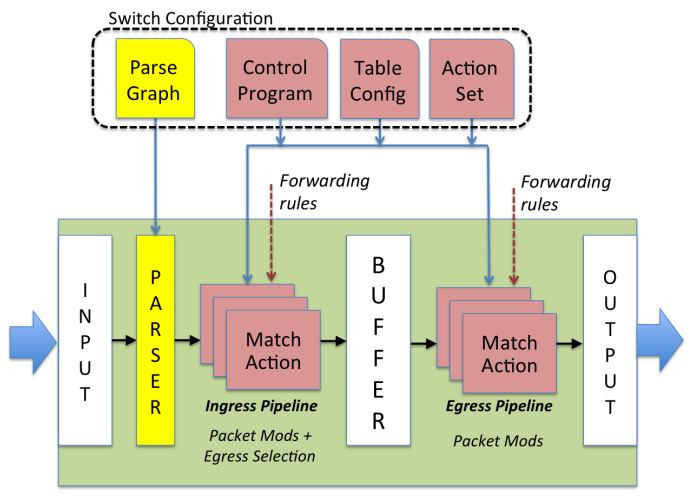
\includegraphics[width=\linewidth]{figures/forwarding_model}
		\caption{The abstract P4 forwarding model. \cite{bosshart2014p4}}
		\label{fig:forwarding_models}
	\end{subfigure}%
	\begin{subfigure}[t]{.5\textwidth}
		\centering
		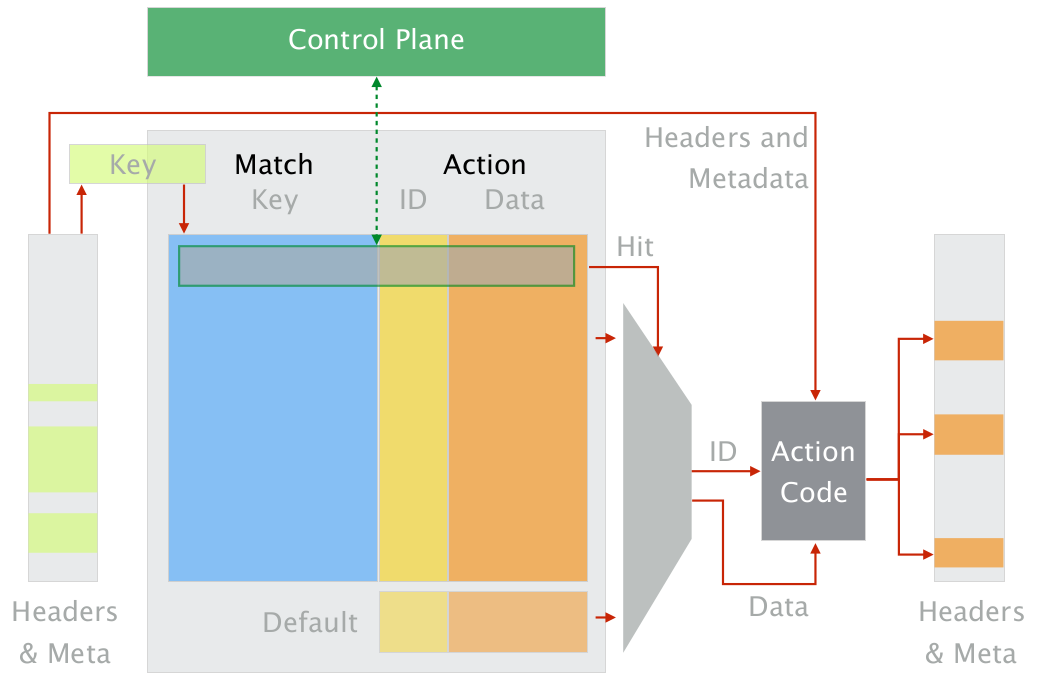
\includegraphics[width=\linewidth]{figures/match_action_tables}
		\caption{Reconfigurable match-action table. \cite{advnet}}
		\label{fig:match_action_tables}
	\end{subfigure}
\end{figure}

\newpage

\noindent The forwarding model is controlled by two types of operations: Configure and Populate. Configure operations program the parser, set the order of match + action stages, and specify the header fields processed by each stage. Configuration determines which protocols are supported and how the switch may process packets. Populate operations add (and remove) entries to the match-action tables that were specified during configuration. Population determines the policy applied to packets at any given time.

\subsection{Language specification}
\subsubsection{Data types}

$P4_{16}$ is a statically typed language with base types and operators to derive composed ones. Base types are:

\begin{center}
	\begin{tabular}{ |c|c| } 
		\hline
		bool & Boolean value \\ 
		\hline
		bit\textless W\textgreater & Bit-string of width W \\ 
		\hline
		int\textless W\textgreater & Signed integer of width W \\ 
		\hline
		varbit\textless W\textgreater & Bit-string of dynamic length $\leq W$ \\
		\hline
		match\textunderscore kind & describes ways to match table keys \\
		\hline
		error & used to signal errors \\
		\hline
		void & no values, used on few restricted instances \\
		\hline
	\end{tabular}
\end{center}
\noindent Note that there are no floats or strings.\newline

Headers are composed operators. Headers are similar to structs in C, containing different fields. Parsing a packet using \texttt{extract()} fills in the fields of the header from a network packet. Headers further have a hidden "validity" field which is set to true upon a successful \texttt{extract()}.

\begin{figure}[hb]
	\centering
	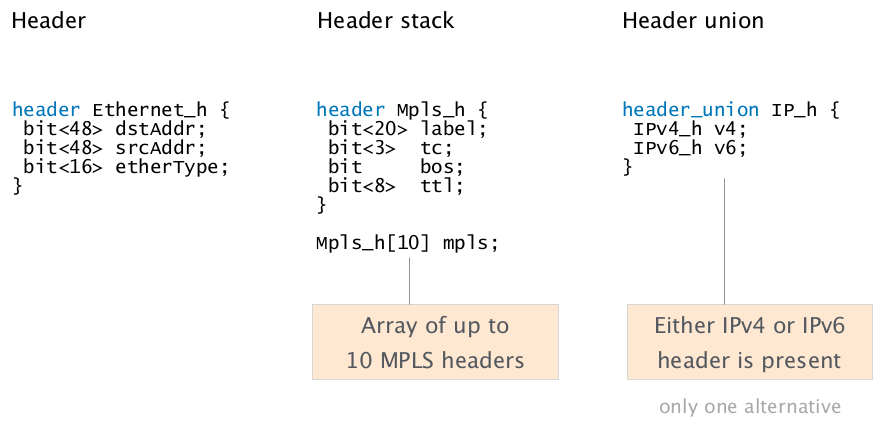
\includegraphics[width=0.75\textwidth,scale=1]{figures/headers}
	\label{fig:headers}
	\cite{advnet}
\end{figure}

\subsubsection{Operations}\label{operations}

P4 operations are similar to C operations and vary depending on the types (unsigned/signed ints, ...). However there is no division or modulo.

Constants, variable declarations and instantiations are pretty much the same as in C too. However, Variables have local scope and their values is not maintained across subsequent invocations. This is due to the fact that the code will be rerun for every new packet. We thus cannot use variables as states since they will be erased for each subsequent run of the code. In order to maintain state, you have to use tables or extern objects.

\subsubsection{Statements}

P4 statements are pretty classical too:  
\vspace{-\topsep}
\begin{itemize}
	\setlength{\itemsep}{0pt}
	\setlength{\parskip}{0pt}
	\item return
	\item exit
	\item \texttt{if()\{...\} else \{...\}} (not in parsers)
	\item \texttt{switch (t.apply.action\_run) \{ a1: \{...\} a2: \{...\}\}} (only in control blocks)
\end{itemize}
\vspace{-\topsep}

\noindent Loops do not exist in P4 (with one exception, see \ref{parser})

\subsection{Parser}\label{parser}

The parser uses a state machine to map packets into headers and metadata. Parsing a header stack requires the parser to loop. This is the only 'loops' that are possible in P4. 

Defining (and parsing) \textit{custom} headers allow you to implement your own protocol. This is why OpenFlow didn't work well in reality and P4 does: with P4, companies can just define their own protocols (for example ETH and UZH can establish a common tunneling protocol). With OpenFlow, companies were either bound to existing protocols and headers or, in case of a influential company, they could bring up new protocols which were eventually implemented in OpenFlow and available to everyone, even though only a small subset of people need that protocol. This led to OpenFlow becoming the overblown beast it is today.

\subsection{Match-action tables}

Match-action tables are the mechanism for performing packet processing. The P4 program defines the fields on which a table may match and the actions it may execute.

\noindent Tables can match on one or multiple keys in different ways:
\vspace{-\topsep}
\begin{itemize}
	\setlength{\itemsep}{0pt}
	\setlength{\parskip}{0pt}
	\item \texttt{exact}: exact comparison (0x01020304)
	\item \texttt{ternary}: compare with mask (0x01020304 \& 0x0F0F0F0F)
	\item \texttt{lpm}: longest prefix match (0x01020304/24)
	\item \texttt{range}: check if in range	(0x01020304 — 0x010203FF)
\end{itemize}
\vspace{-\topsep}

\noindent Table entries are added through the control plane.\newline
Example: \texttt{table\_add ipv4\_lpm ipv4\_forward 1.2.3.0/24 => 01:01:01:01:01:01 1}

The match-action tables are divided between ingress and egress. While both may modify the packet header, ingress match-action determines the egress port(s) and determines the queue into which the packet is placed. Based on ingress processing, the packet may be forwarded, replicated (for multicast, span, or to the control plane), dropped, or trigger flow control. Egress match-action performs per-instance modifications to the packet header – e.g., for multicast copies.

Packets can carry additional information between stages, called metadata, which is treated identically to packet header fields. Some examples of metadata include the ingress port, the transmit destination and queue, a timestamp that can be used for packet scheduling, and data passed from table-to-table that does not involve changing the parsed representation of the packet such as a virtual network identifier.

\subsection{Actions}

Actions are blocks of statements that possibly modify the packets (think of them as functions in C). P4 supports the construction of complex actions from simpler protocol-independent primitives. Actions can either be invoked from within a control block or as a result of a match in a match-\textit{action}-table.

\newpage

\noindent Actions that are invoked from within a control block take directional parameters, indicating how the corresponding value is treated within the block.
\vspace{-\topsep}
\begin{itemize}
	\setlength{\itemsep}{0pt}
	\setlength{\parskip}{0pt}
	\item \texttt{in}: parameters in only read inside the action (like parameters to a function)
	\item \texttt{out}: parameter is uninitialized and will be written to inside the action (like return values)
	\item \texttt{inout}: combination of in and out (like “call by reference”)
\end{itemize}


\noindent Action parameters resulting from a table lookup do not take a direction as they come from the control plane.

\subsection{Control flow}

Control flow consists of various concepts, for an extensive list, please consider \cite{p416spec}. Some basic concepts are:
\vspace{-\topsep}
\begin{itemize}
	\setlength{\itemsep}{0pt}
	\setlength{\parskip}{0pt}
	\item applying a table: \texttt{ipv4\_lpm.apply()}
	\item Checking if there was a hit: \texttt{if (ipv4\_lpm.apply().hit) \{...\}}
	\item Check which action was executed: \texttt{switch (ipv4\_lpm.apply().action\_run) \{...\}}
\end{itemize}

\noindent Other often used concepts are: 
\vspace{-\topsep}
\begin{itemize}
	\setlength{\itemsep}{0pt}
	\setlength{\parskip}{0pt}
	\item re-computing checksums (needs to be done when changing a packet, otherwise the kernel will drop packets upon checksum mismatch)
	\item cloning packets
	\item sending packets to control plane (using dedicated Ethernet port, or target-specific mechanisms (e.g. digests))
\end{itemize}













\label{lastpage} % this must stay here
\clearpage
\addcontentsline{toc}{section}{References}
\bibliographystyle{acm}
\bibliography{refs}

\clearpage
\appendix
\pagenumbering{Roman}

\end{document}
